%%%%%%%%%%%%%%%%%%%%%%%%%%%%%%%%%%%%%%%%%%%%%%%%%%%%%%%%%%%%%%%%%%%%%%%%
\chapter{Magnetic Resonance Imaging} \label{chap:MagneticResonanceImaging}
%%%%%%%%%%%%%%%%%%%%%%%%%%%%%%%%%%%%%%%%%%%%%%%%%%%%%%%%%%%%%%%%%%%%%%%%
\vspace{1cm}

Magnetic resonance imaging (MRI) is one of the most powerful and versatile techniques in modern medical imaging. Its non-invasive nature and the absence of ionizing radiation have established it as a cornerstone in both clinical diagnostics and biomedical research. MRI exploits the fundamental physical interactions between nuclear spins and magnetic fields, providing not only high-resolution structural images, but also access to functional, metabolic, and microstructural information.

This chapter goes through the fundamental concepts of MRI. First, it introduces the underlying physical principles of nuclear magnetic resonance, including spin dynamics, relaxation processes, and signal generation. Second, it describes how spatial encoding is achieved through magnetic field gradients, which allow the reconstruction of three-dimensional images.

\section{Physical Principles}
Magnetic resonance imaging (MRI) is based on the fundamental physical phenomenon of nuclear magnetic resonance (NMR), first demonstrated experimentally by I.\ Rabi in 1938 and later independently verified by Purcell and Bloch in 1946\,\cite{NMR}. NMR describes the resonant interaction between the intrinsic magnetic moment of atomic nuclei and external magnetic fields. This effect enables the observation of nuclear spin behavior through the emission of electromagnetic radiation, providing the physical foundation for MRI, a technique capable of generating high-resolution, non-invasive images of biological tissues.

If a nucleus possesses an intrinsic angular momentum, or spin \vect{I}, the associated magnetic dipole moment is:
\begin{equation}
    \bm{\upmu} = \gamma \vect{I},
\end{equation}
where $\gamma$ is the gyromagnetic ratio, a constant depending on the nucleus species. Only nuclei with a nonzero spin quantum number can exhibit magnetic resonance. Actually, nuclei with a integer spins are not able to produce detectable signals in MRI, because their gyromagnetic ratios are much smaller than those of half-integer spins. Among them, in biological tissues, the hydrogen nucleus ($^1$H) is the most suitable for MRI because of its high abundance in water and lipids and its relatively large $\gamma$, which yields strong detectable signals.

The result of an observation of the $z$-component of the angular momentum \vect{I} of a single nucleus in its ground state is an integer or half-integer number $m$ ranging from $-I$ to $+I$, in steps of \num{1}. Thus, $m$ can assume $2I + 1$ distinct values, which implies $2I + 1$ possible values for the measurement of the $z$-component of the magnetic moment
\begin{equation}
    \mu_z = \gamma \hbar m,
\end{equation}
where $\hbar$ is the reduced Planck constant.

Each value of $m$ corresponds to a specific energy level of the nucleus. When a magnetic field $\vect{B_0}$ is applied, these energy levels split due to the Zeeman effect, resulting in a set of discrete energy states. The energy associated with each state is given by
\begin{equation}
    E_m = -\gamma \hbar m B_0.
\end{equation}
In case of $^1$H, which has $I = \frac{1}{2}$, the two possible values of the magnetic moment correspond to $m = +\frac{1}{2}$ and $m = -\frac{1}{2}$. This results, in turn, in two distinct energy states separated by $\Delta E = \gamma \hbar B_0$. The presence of discrete energy levels generates an observable quantity named magnetization \vect{M}, which is defined as
\begin{equation}
    \vect{M} = N \gamma \hbar (\langle I_x \rangle \vect{i} + \langle I_y \rangle \vect{j} + \langle I_z \rangle \vect{k}),
\end{equation}
where $N$ is the number of nuclei with nonzero spin, and $\langle \cdot \rangle$ denotes the expectation values of the nuclear spin components along the axes. At relatively low temperature $T$ (even room temperature) and high magnetic field \vect{B_0}, the magnetization obeys Curie's law\,\cite{curie_law}:
\begin{equation}
    \vect{M} = N\frac{\gamma^2 \hbar^2 I(I+1)}{3\mathrm{k}_\mathrm{B} T} \vect{B_0},
\end{equation}
where $\mathrm{k}_\mathrm{B}$ is the Boltzmann constant. It is important to notice that stronger magnetic fields or lower temperatures increase the detectable magnetization.

The last fundamental principle of NMR is a phenomenon, known as Larmor precession, which originates from the application of an external magnetic field to nuclei with nonzero spin. The magnetic moments $\bm{\upmu}$ of the nuclei will not just align with the magnetic field, but they will describe a conical motion around \vect{B_0} (Fig.\,\ref{fig:larmor_precession}), at the Larmor frequency:
\begin{equation}
    \nu_\textrm{L} = \frac{\omega_\textrm{L}}{2\uppi} = \frac{\gamma B_0}{2\uppi}.
\end{equation}
To perturb the equilibrium state and generate a measurable signal, a second oscillating magnetic field \vect{B_1}, also called radiofrequency (RF) pulse, is applied perpendicularly to \vect{B_0}. If the oscillation frequency of \vect{B_1} matches $\omega_\mathrm{L}$, resonance occurs and the nuclei absorb energy, undergoing transitions between the energy levels. As a consequence, a nutation angle appears, which increases with the pulse duration, causing the magnetization \vect{M} to tilt away from the $z$-axis by a flip angle, defined as
\begin{equation}
    \alpha = \gamma B_1 t,
\end{equation}
where $t$ is the duration of the RF pulse. Typical pulses of \qty{90}{\degree} or \qty{180}{\degree} rotate the magnetization fully into the transverse plane or invert it, respectively.

\begin{figure}[htbp]
    \centering
    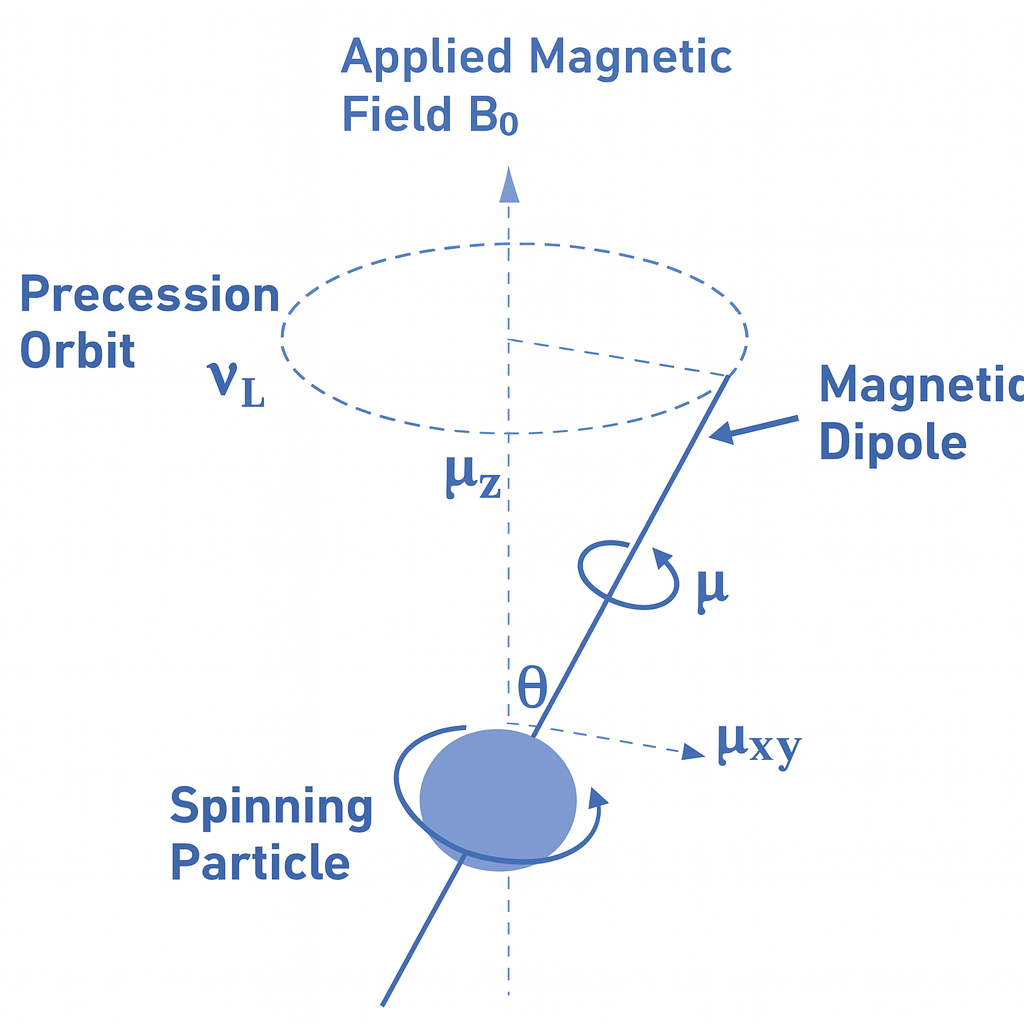
\includegraphics[width=0.45\textwidth]{figures/larmor_precession.png}
    \caption{Larmor precession of a nuclear spin in a magnetic field. © 2025 Science Info, from \cite{science_info}.}
    \label{fig:larmor_precession}
\end{figure}

\section{Relaxation and Signal Generation}
Once that the RF pulse has ended, \vect{M} returns to the previous equilibrium state around \vect{B_0}; this induces a voltage in the receiver coil, which is the measurable NMR signal. The return to the equilibrium is not instantaneous, but it occurs through two distinct relaxation processes, characterized by different time constants and both governed by the Bloch equations. These processes are crucial for determining the contrast in MRI images, as they affect the temporal evolution of the magnetization components.

\paragraph{Transverse Relaxation.}
Also known as spin-spin relaxation or T2 relaxation, the transverse relaxation is an entropic process that denotes the progressive loss of phase coherence among spins. It manifests as an attenuation of the observable transverse magnetization. Following the excitation imparted with the RF field \vect{B_1}, the transverse component of the magnetization $M_{xy}$ decays because relative phases disperse over time, as illustrated in Fig.\,\ref{fig:transverse_relaxation}. Two principal mechanisms are implicated:
\begin{description}
  \item[Spin-spin interactions] Stochastic dipolar couplings and molecular motion induce local frequency perturbations that irreversibly randomize relative phases, giving rise to the intrinsic decay constant $T_2$.
  \item[Static field inhomogeneities] Spatial variations in magnetic susceptibility within the specimen perturb the applied field \vect{B_0}. These distortions---whose magnitude depends on tissue composition and geometry---generate a rapid, position-dependent dephasing of nucleus spins. Refocusing methods---e.g., spin echoes---can largely reverse the effects of this dephasing factor.
\end{description}
Collectively, these effects produce a distribution of phases across groups of nuclei: individual spins may continue to precess near $\omega_0$, yet their vector sum---i.e., the measurable transverse magnetization---decays toward zero.

The Bloch equation for the transverse magnetization component $M_{xy}$ is
\begin{equation}
  M_{xy}(t) = M_{xy}(0)\,\mathrm{e}^{-\frac{t}{T_2}},
\end{equation}
where $M_{xy}(0)$ is the transverse magnetization immediately after the end of the RF pulse. The time constant $T_2$ characterizes the rate of decay due to spin-spin interactions. Here the effects of static field inhomogeneities are not included; when they are, the effective decay constant is $T_2^*$, defined by
\begin{equation}
    \frac{1}{T_2^*} = \frac{1}{T_2} + \frac{1}{T_\text{inh}},
\end{equation}
where $T_\text{inh}$ accounts for the inhomogeneity effects.

\begin{figure}[htbp]
    \centering
    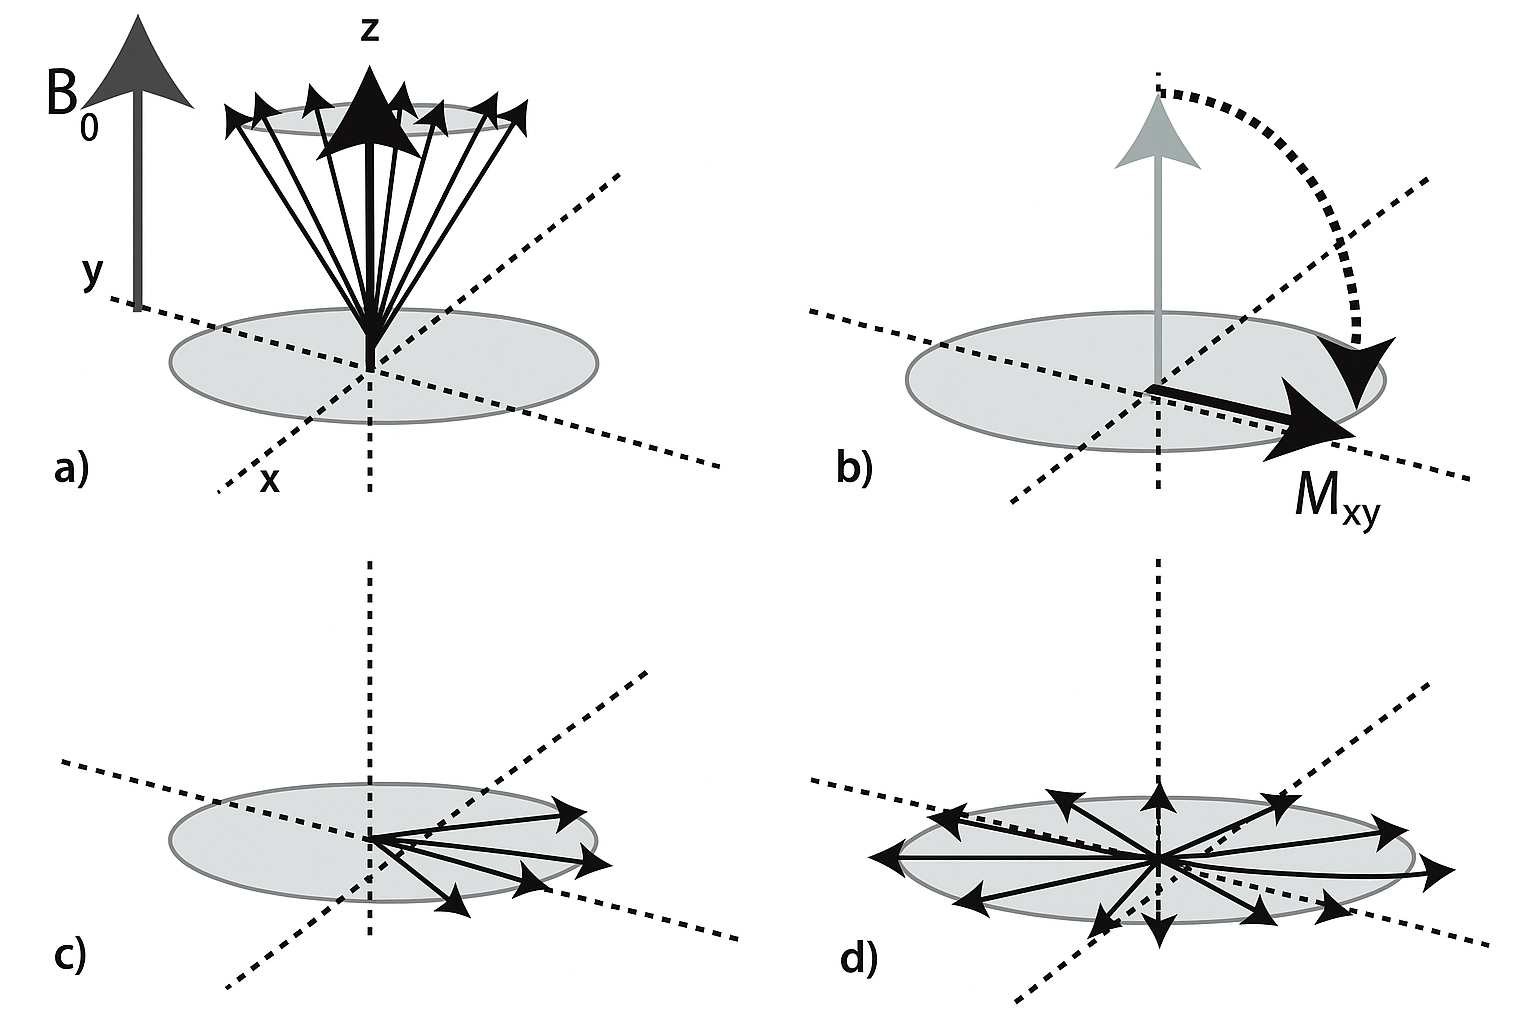
\includegraphics[width=0.65\textwidth]{figures/transverse_relaxation.png}
    \caption{Transverse relaxation of nuclear spins. © 2025 Informa UK Limited, from \cite{Lanting2010}.}
    \label{fig:transverse_relaxation}
\end{figure}

\paragraph{Longitudinal Relaxation.} Also known as spin-lattice relaxation or T1 relaxation, the longitudinal relaxation describes the recovery of the longitudinal magnetization component $M_z$ as energy is exchanged between the spin system and its surrounding molecular environment, that is, the lattice. Once that RF excitation ended, $M_z$ reappears, returning toward its thermal equilibrium value $M_0$. This process is governed by the Bloch equation for the longitudinal magnetization:
\begin{equation}
    M_z(t)=M_z(0)\,\mathrm{e}^{-\frac{t}{T_1}}+M_0 \left(1-\mathrm{e}^{-\frac{t}{T_1}} \right),
\end{equation}
where $M_z(0)$ is the longitudinal magnetization immediately after the end of the RF pulse. $T_1$ depends on field strength, viscosity and temperature, and typically satisfies $T_1>T_2$ in biological tissues.

The relaxation times $T_1$ and $T_2$ vary significantly among different tissue types, providing the basis for image contrast in MRI (see Fig.\,\ref{fig:relaxation_plots}). By selecting appropriate timing parameters for the RF pulses and signal acquisition---e.g., the repetition time (TR) and echo time (TE)---the image contrast can be manipulated to highlight specific tissues. As a general rule, short TR and TE values yield T1-weighted images, emphasizing differences in longitudinal relaxation, while long TR and TE values produce T2-weighted images, dominated by transverse relaxation. When TR is long and TE is short, the resulting images are proton-density-weighted, reflecting variations in hydrogen concentration. The aforementioned weighting techniques are schematically illustrated in Fig.\,\ref{fig:weightings}.

\begin{figure}[htbp]
    \centering
    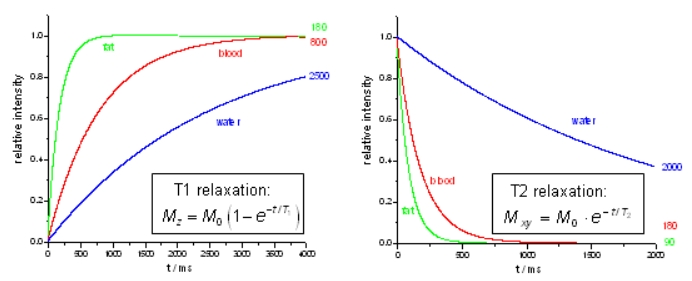
\includegraphics[width=0.95\textwidth]{figures/relaxation_plots.jpeg}
    \caption{Bloch equations for T1 (left) and T2 (right) relaxations in different biological tissues. © 2025 Heinrich-Heine-Universität Düsseldorf, from \cite{hhu}.}
    \label{fig:relaxation_plots}
\end{figure}

\begin{figure}[htbp]
    \centering
    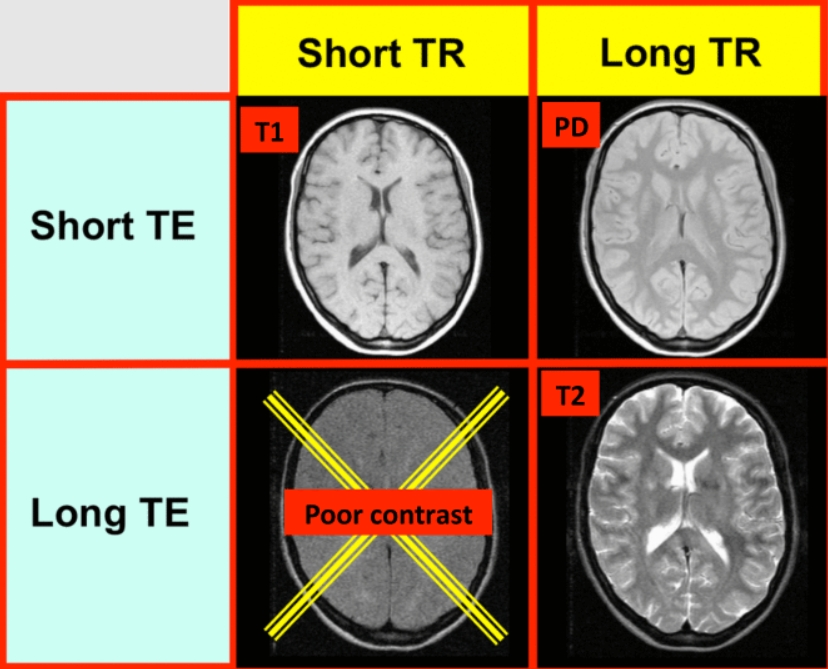
\includegraphics[width=0.6\textwidth]{figures/weightings.jpeg}
    \caption{Relationship between the timing parameters TR and TE, and the T1, T2, and proton density weightings. © 2025 AD Elster, from \cite{mri_questions}.}
    \label{fig:weightings}
\end{figure}

\section{Spatial Encoding}
